\chapter{How old is a star clusters}

%TODO after setting "log", tell them that you can right-click and drag vert and horiz to adjust the brightness scale

\section{Introduction}

In this lab you will use a Hertzsprung-Russell (H-R) Diagram to learn about a star cluster. This will give us insight into the stellar populations in the clusters we observe, and allow us to estimate the age of their constituent stars. 

\section{Learning goals}

\begin{itemize}
    \item Gain an understanding of astronomical observation, image analysis and photometry
	\item Gain practice performing basic calculations on datasets and making informative scientific figures from those data
	\item Retrieve data from astronomical databases.
	\item Learn where different stellar populations lie on the HR diagram, and understand the physical reasons behind these localizations
	\item Estimate stellar cluster ages using the predictions of stellar evolutionary models. 
\end{itemize}

\textbf{Rubric rows to focus on:} D1, D4, F1, F2, G2, G4, G5

\section{Scientific background}

Stars evolve (i.e., change their properties) over millions and often billions of years – too slow for us to see the evolution over a human lifespan.  Such impressive longevity is due to the fact that stars are powered by thermonuclear reactions, which are very efficient in generating abundant energy and have quite a bit of fuel to last for a long time. Stars like our Sun last about 10 billion years (so the Sun is in its middle age). The long timescale of evolution also means that we have to develop a different way to study stellar evolution. 

Astronomers explore evolution of stars by observing large populations of stars where different stars are in different stages of evolution. Of course, in order to do this we need to be able to tell which star is in what stage. This is done by a combination of observations – which measure luminosity and surface temperatures – and theoretical models – which predict how luminosity and surface temperature change as stars evolve. The key is that luminosity and temperature at a certain age are determined by star's mass, chemical composition, and details of thermonuclear reactions (which elements are burning, over what fraction of star's volume, etc.).

Luminosity and temperature of stars are related because they are both determined by their internal structure, which, in turn, is determined by the basic physical properties (mass, chemical composition, age). Therefore, stars are not scattered randomly in the luminosity and temperature space but follow well-defined sequences, which reflect the ranges of the controlling parameters in a given stellar population. 

The surface temperatures of stars can be deduced by fitting a blackbody radiation spectrum to their spectra. Even for stars that do not have spectra measured, their temperatures can be deduced from their colors (Recall: does bluer color correspond to cooler or hotter temperature?). Our eyes and brain perceive color by analyzing spectral composition of the incoming light. In astronomy, a star's color is defined as the difference between its magnitudes measured through two different filters that block out all light except light within a fairly narrow range of wavelengths. 

In order to interpret evolutionary states, we look at physical groupings of stars called stellar clusters, which are located at the same distance from us and were born at the same time from the same cloud of dense gas. The spread in their properties will thus not be due to different ages or initial compositions, but mainly due to different masses. As you will see, stars occupy distinct regions of the observable equivalent of the luminosity-temperature space --- the magnitude-color space called the Hertzsprung-Russell (H-R) diagram. We will make this diagram for a star cluster.

\subsection{Filters}
Light is composed of energy-packets termed \textbf{photons} with energies that determine their wavelengths (sorter wavelength $\implies$ higher energy). Thus every light source exhibits a \textbf{spectrum} of energies based on its components, which are determined by the physics of the light emission process. Observing the spectrum of radiation emitted from astronomical objects is a fundamental tool in observational astrophysics. However, obtaining the specific intensity of radiation as a function of energy for many dim sources is challenging. An easier way to asses the electromagnetic energies observed is to image them in different \textbf{filters}: materials placed at the opening of a telescope that are transparent to a known range of wavelengths and opaque to all others (thus ``filtering'' the light). Thus, one can image the same object with multiple different filters to get a sense of the wavelength regimes that dominate the light from a source.

A filter is characterized by its \textbf{transmission function}: a function that characterizes the amount of light that is transmitted by the filter at each wavelength. Figure~\ref{sdss_filters} shows the transmission functions for some standard astronomical filters (similar to the one's you'll be using in this class).

\begin{figure}
\label{sdss_filters}
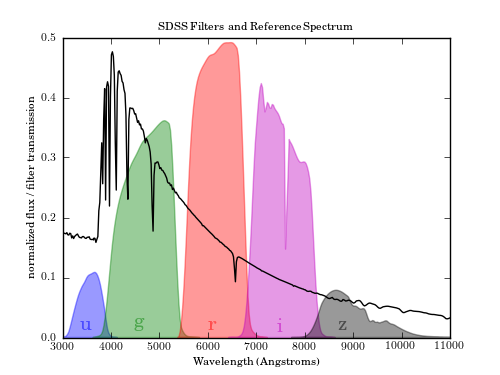
\includegraphics{hr_diagram/fig_sdss_filters_1.png}
\caption{Filter Transmission Functions for the Sloan Digetal Sky Survey, overlaid on a stellar spectrum. The magnitude observed by each filter will be proportional to the integrated spectrum multiplied by the filter transmission. It's clear in this image that the underlying spectrum of the star will cause the different filters to have different magnitudes. Image source: \texttt{http://www.astroml.org/\_images/fig\_sdss\_filters\_1.png}}
\end{figure}

\section{Defining color}

Since different bands measure brightness in different wavelengths, the ratio of flux in two bands is a measure of an object's color. Therefore, the difference between astronomical magnitudes of an object in different bands is a measure of its color, since the magnitude scale is logarithmic:

\begin{equation}
m_A - m_B = -2.5\log\left(\frac{F_A}{F_B}\right).
\end{equation}

An H-R diagram is a plot of stellar magnitude vs. color - aka a ``color magnitude diagram''. A star's color is an observational indication of it's surface temperature. Since all of the stars in a star cluster are at approximately the same distance, their apparent magnitude gives a good relative indicator of luminosity. Therefore, a color-magnitude diagram of stars at roughly constant distance is effectively a temperature-luminosity diagram, and stars fall in characteristic regions of this parameter space based on their mass, age, and metallicity.

We will have data in two wavelength bands, so we can subtract those magnitudes to get a color index. With the software or coding language of your choice, you will plot $g$ on the vertical axis and $g - r$ on the horizontal axis.
%Add error bars to your plot. If doing so for each data point becomes crowded on your figure, you can estimate a typical error from your data and include it in a legend. 

\section{Making an HR Diagram}

To learn about a star cluster, you'll make a color-magnitude diagram of the stars in that cluster. You'll be analyzing M15, a globular star cluster in the Pegasus constellation. To make the diagram, you need magnitudes in at least two different filters for many stars in the cluster. Since this would be incredibly time-consuming to do by hand, you will retrieve this information from an online database.

\begin{steps}
	\item Open the SkyServer Search Form in a browser: \url{http://cas.sdss.org/dr7/en/tools/search/form/Default.aspx}.
	
	\item Select "Show me [stars] in the region [around:]". Note that you will need to know the celestial coordinates of the part of the sky that you want retrieve data about, as well as the radius of a circle that captures all the objects you want.
	
	\item Look up M15 in Stellarium and record its RA and Dec (J2000 values). It may be helpful to turn off the ground and atmosphere to get a better view. Then, determine a radius in arcminutes that includes all of the cluster. You can either use the Field Of View (FOV) listed on the screen, or you can turn on the Equatorial Grid by selecting that option in the bottom toolbar or pressing 'e' and use the contour lines.
	
	\item The Search Form wants the RA and Dec in decimal degrees. So convert the RA and Dec that you recorded to decimal degrees and enter this (for example, an RA of 15h30m20s converts to 232.5833 degrees). You can use this website to assist: \url{https://www.swift.psu.edu/secure/toop/convert.htm}.
	
	\item In the Form, tell it to output 1000 objects, and the magnitudes of the objects.
	
	\item Select ``Generate'' or ``Update Query'' and it will convert all the options into a database query that you should then ``Submit''. This opens a new tab with the output from the query.
	
	\item If the outcome from the query has much fewer than 1000 objects, then increase the radius (and/or check to ensure you have the correct RA and Dec entered).
	
	\item Once you have lots of objects, change the form to output a CSV file.
	
	\item Plot the data from the CSV file using your favorite spreadsheet or programming environment. Specifically plot 'g' vs. 'g-r', with 'g' on the vertical axis, as a scatter plot.

	\item Label the different stages of stellar evolution on your plot.
\end{steps}

\section{Comparing to stellar evolution models}

The last portion of this lab involves estimating the age of these stellar populations by comparing their color magnitude diagrams with predictions from a stellar evolution model. Stellar physics is sufficiently well-understood that accurate evolutionary models have been constructed to calculate the observable properties of stars across their lifetimes. Because stars evolve in their position on the HR diagram, we can estimate the age of our observed cluster by comparing these models to our observations.

Several files containing model predictions for the magnitudes of stars at different ages are contained in files on the course website. These have been calculated using the observed metallicity of the star cluster to predict the positions of stars at ages $10^7$, $10^8$, $10^9$, and $10^{10}$ years. These are called isochrones - stellar properties as a function of stellar mass for a fixed age (and metallicity). Note that these magnitudes were calculated using prior knowledge of the star cluster metallicity, and have been corrected for cluster distance and extinction due to intervening galactic dust (taken from \cite{DurrellHarris1993} for M15 and \cite{Currie2010} for NGC 869).

\begin{steps}
	\item Plot these isochrones on your H-R diagrams and compare them to your data to estimate the cluster age. Be sure to estimate an error on this value and explain your method in your lab report.
	
	\item What changes in stellar properties are represented by the different locations of isochrones of different ages?
	
	\item What physical processes occuring inside the star underlie those changes?
\end{steps}

\section{Report checklist and grading}

Each item below is worth 10 points, and there is an additional 10 points for attendance and participation. See Appendix\ \ref{cha:lab-report-format} for guidance on writing the report and formatting tables and graphs.

\begin{enumerate}
	\item The coordinates of M15 and the radius you choose, along with how you found these (Step 3).
	
	\item The plot of $g$ vs. $g-r$ with labels of different stages of stellar evolution (Steps 9--10).
	
	\item Plot of H-R diagram with isochrones (Step 11).
	
	\item Analysis and determination of cluster age, with uncertainty (Step 11).
	
	\item Answers to questions in Steps 12--13.
\end{enumerate}